\chapter{Objetivos}
\label{cap:capitulo2}


En esta sección se describirá el problema a resolver junto con los objetivos y requisitos pautados en el desarrollo del TFG


\section{Descripción del problema}
\label{sec:descripcion}

El objetivo principal de este TFG, es desarrollar un comportamiento de navegación autónoma basado en 
aprendizaje por refuerzo e inteligencia artificial, en el que el dron sea capaz de navegar de una manera robusta sin colisiones por escenarios urbanos. El enfoque de este trabajo de investigación 
se centra en la creación de una solución eficiente y completa ante la problemática que puede llegar a tener la navegación autónoma, se 
muestra un comportamiento capaz de realizar el seguimiento de un carril para demostrar la complejidad de mantener una trayectoria estable 
y precisa utilizando un dron. 

A continuación, se definen los siguientes subobjetivos: 

\begin{enumerate}
    \item Estudio del arte de los drones con el objetivo de definir las posibilidades que puede ofrecer y definir 
    la navegación autónoma dentro del entorno en el que se desarrollará el TFG. 
    \item Análisis y desarrollo de un sistema perceptivo basado en redes neuronales en la navegación autónoma de drones.
    \item Desarrollo  de un sistema de control para drones utilizando técnicas de aprendizaje por refuerzo para lograr una navegación 
    autónoma, segura y eficaz.
    \item Análisis y desarrollo de una aplicación de navegación autónoma de drones basándonos en el seguimiento de un carril.
    \item Análisis y comparativas de los diferentes comportamientos desarrollados en este trabajo con el fin de 
    lograr resultados interesantes acerca de la utilización de redes neuronales y aprendizaje por refuerzo en la navegación autónoma de drones.
\end{enumerate}
\newpage
\section{Requisitos}
\label{sec:requisitos}

Los requisitos que han de cumplirse en este trabajo son: 
\begin{enumerate}
    \item Uso del vehículo UAV en el entorno de simulación fotorrealista Airsim junto a UnRealEngine.
    \item Utilización del middleware robótico ROS para así garantizar la interoperabilidad del trabajo en otro tipo de escenarios permitiendo
    la reutilización del proyecto en diversas aplicaciones. 
    \item Comportamiento robusto y en tiempo real para garantizar la navegación segura del vehículo dentro del circuito urbano.
    \item Los sistemas desarrollados deben ser reactivos para poder reaccionar a su entorno de manera concisa y eficiente durante
    la navegación.
    \item Emplear el algoritmo de Q-learning para la navegación autónoma del dron. 
\end{enumerate}


\section{Metodología}
\label{sec:metodologia}

Este trabajo, comenzó oficialmente en Septiembre del 2023 aunque en Diciembre del 2022 se plantearon varias ideas a desarrollar, y se finalizó en Mayo del 2024. \\

La metodología que se llevo a cabo fue:

\begin{enumerate}
    \item Reuniones semanales mediante Teams\footnote{\url{https://www.microsoft.com/es-es/microsoft-teams/group-chat-software}} con una duración de media o una hora, con el fin de tener un control semanal y pactar los objetivos semanales a seguir. Gracias a estas reuniones, se tenia una organización global del proyecto. 
    \item Contacto vía email de la universidad con el fin de solventar problemas urgentes. 
    \item Utilización de la metodología Kanban\footnote{\url{https://canalinnova.com/que-es-y-para-que-sirve-el-kanban-definicion-fases-y-pasos/}}: Este tipo de metodología consiste en crear un flujo de trabajo
    en equipos mediante la gestión visual. Se compone de varias fases:
  
    \begin{itemize}
      \item \textbf{Fase 1: Inicio del proyecto}. Consiste en marcar los objetivos que se deben seguir dentro del proyecto junto la asignación e identificación de tareas. En esta fase, 
      definimos el tipo de aplicación que se iba a seguir que es la navegación autónoma de drones considerando un entorno de simulación de carreteras, la infraestructura, los tipos 
      de algoritmos a seguir y las analíticas de los comportamientos desarrollados durante el TFG. \newline
      \item \textbf{Fase 2: Diseño del tablero Kanban}. Se crea un tablero en donde se visualizarán las tareas y su estado. Cada tarea se definen en las columnas del tableros las
      tareas que se deben realizar junto con indicadores visuales como se muestra en la figura \newline
      \item \textbf{Fase 3: Implementación del tablero Kanban}. Se asignan las tareas a realizar y se establecen límites de trabajo en progreso como el tiempo de desarrollo para 
      completar dicha tarea. \newline
      \item \textbf{Fase 4: Seguimiento y mejora continua}. Se realiza un flujo continuo y constante del trabajo identificando nuevas soluciones para mejorar la eficacia y la 
      productividad hasta de poder cambiar estrategias existentes por nuevas alternativas previamente definidas. En este trabajo hemos realizo varias tareas y seguimientos para encontrar
      la mejor solución ante el problema a resolver.\newline

      
      A lo largo del desarrollo de este TFG, se marcaron estas 4 fases permitiendo cambios y mejoras continuas hasta llegar al resultado final.

    \end{itemize}
  
    \begin{figure} [H]
        \begin{center}
          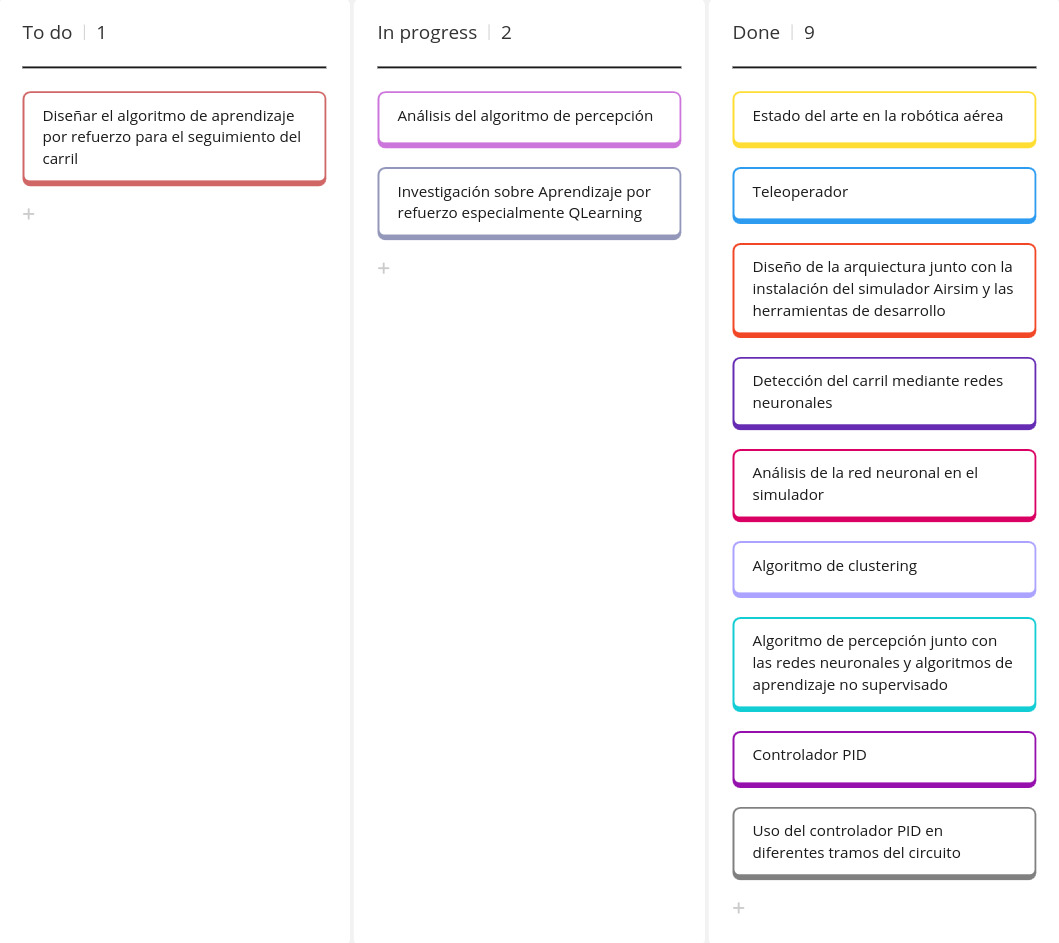
\includegraphics[scale=0.4]{figs/objetivos/Kanban3.jpg}
        \end{center}
        \caption{Ilustración del tablero Kanban durante el desarrollo del TFG}
        \label{fig:Espiral}
      \end{figure}
  
    \item Tener un control de versiones mediante la plataforma GitHub\footnote{\url{https://github.com/RoboticsLabURJC/2022-tfg-barbara-villalba}}, con el objetivo de tener un almacenamiento de código y respaldos de ello.  
    \item El uso de un blog \footnote{\url{https://roboticslaburjc.github.io/2022-tfg-barbara-villalba/}}, en el cual se describió brevemente los pasos que se siguieron para el desarrollo del TFG.
\end{enumerate}

\begin{figure} [H]
    \begin{center}
      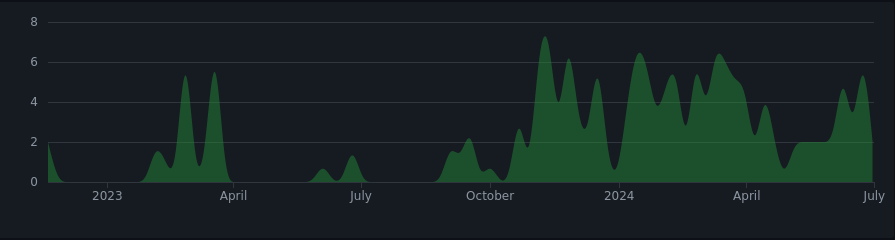
\includegraphics[width=0.9\textwidth,height=0.3\textwidth]{figs/objetivos/github.png}
    \end{center}
    \caption{Seguimiento de trabajo en GitHub}
    \label{fig:github}
  \end{figure}


\section{Plan de trabajo}
\label{sec:plantrabajo}

Finalmente, los pasos a seguir de este trabajo han sido: 
\begin{enumerate}
    \item Comienzo del trabajo. 
    \begin{itemize}
        \item Búsqueda del problema a desarrollar y análisis del estado del arte del uso de los drones en aplicaciones robóticas.
        \item Instalación de las diferentes librerías y aplicaciones de software. 
        \item Preparación de configuración de toda la infraestructura, teniendo un análisis y estudio de comunicaciones para poder comenzar con el desarrollo. 
    \end{itemize}
    \item Desarrollo: Una vez se tuvo listo toda la infraestructura tanto de comunicaciones como de librerías de software, se dio a pie el comienzo del desarrollo del código
        \begin{itemize}
            \item En primer lugar, se desarrollo un teleoperador sencillo del drone para ver el funcionamiento del vehículo y dicho comportamiento.
            \item Una vez finalizada la tarea del teleoperador, se comenzó con los algoritmos de percepción de detención de carril mediante redes neuronales.
            \item Análisis y comparación de los resultados de los diferentes modelos que ofrece la red neuronal escogida con el propósito de tener la mejor solución. 
            \item El siguiente paso fue estudiar la posibilidad de tener un algoritmo de aprendizaje no supervisado llamado clustering para clasificar las diferentes lineas que aparezcan en el escenario de la carretera.
            \item Desarrollo del algoritmo de percepción junto con los dos puntos anteriormente mencionados.
            \item Con el fin del algoritmo de percepción, se comenzó el desarrollo de un controlador sencillo PID para ver el funcionamiento de la percepción y de la navegación en el vehículo. 
            \item A continuación, fue la programación del algoritmo de aprendizaje por refuerzo para el seguimiento del carril.
        \end{itemize}
    \item Evaluación: Se realizo la comparativa de los resultados obtenidos en el aprendizaje por refuerzo.
        
    \item Redacción de la memoria del trabajo para la documentación de todo el proceso de investigación realizado. 
\end{enumerate}


